\documentclass[a4paper,10pt]{article}
\usepackage[utf8]{inputenc}
\usepackage[spanish]{babel}
\usepackage{graphicx}
\usepackage{epstopdf}
\usepackage{graphicx}
\usepackage{listings}
\usepackage{array}
\usepackage{hyperref}
\usepackage[margin=25mm]{geometry}

\title{Documento de Diseño de Air Guitar}
\author{Carlos Bergen Dyck \and Gustav Svensk}
\begin{document}

\renewcommand{\arraystretch}{1.5}
\maketitle
\begin{center}
        {\large Versión 0.1}
\end{center}
\newpage


\section{Prefacio}
\begin{tabular}{p{3cm} p{12cm}}
        & Este es el Documento de Diseño de Air Guitar, que consiste en
        producir sonido cuando se toca a su Air Guitar. \\
        \textbf{Alcance del documento} & El Documento de Diseño presenta las
        decisiones de diseño de Air Guitar. Describe los siguientes aspectos del
        sistema: arquitectura revisada, descripción de cada módulo, y diseño
        detallado de cada función incluyendo sus casos de prueba.\\
        \textbf{Documentos relacionados} & Documento de Requisitos de Air Guitar,
        versión 0.1, 6/11/2013. \\
        \textbf{Autor} & Carlos Bergen Dyck y Gustav Svensk \\
        \textbf{Lectores} & Este documento está dirigido principalmente a los
        desarrolladores del proyecto, pero es de interés de todos los
        interesados en como se implementa el proyecto. \\
        \textbf{Aprobación} & Este documento debe ser sometido a revisión de
        pares, pero no tiene una aprobación formal por alguien externo al equipo
        de desarrollo.
\end{tabular}

\section{Historia del Documento}
\begin{tabular}{|c|c|p{6cm}|p{4cm}|}
        \hline
        \textbf{Versión} & \textbf{Fecha} & \textbf{Explicación del cambio} &
        \textbf{Autor} \\ \hline
        0.1 & 25/11/2013 & Primer borrador & Carlos Bergen Dyck y Gustav Svensk \\
        \hline
\end{tabular}

\newpage
\tableofcontents

\listoftables

\listoffigures
\newpage

\section{Arquitectura Revisada del Sistema}
En el Documento de Requisitos de Nombre del Sistema se especificó su
arquitectura inicial. A la luz de un trabajo de diseño más detallado, aquí se
presenta la arquitectura definitiva, que incluye más detalle y posiblemente
algunos cambios.
\subsection{Diagrama de Contexto}
El diagrama de contexto se puede ver en figura~\ref{fig:contexto}.
\begin{figure}[h]
        \centering
        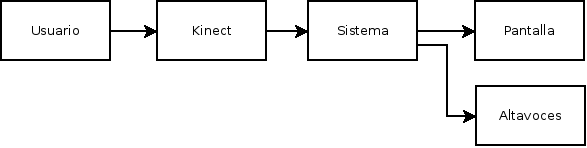
\includegraphics[width=0.8\textwidth]{../imagenes/diagrama_de_contexto.png}
        \caption{Diagrama de Contexto}
        \label{fig:contexto}
\end{figure}

\subsection{Diagrama de Arquitectura}
El diagrama de arquitectura se puede ver en figura~\ref{fig:arquitectura}
\begin{figure}[h]
        \centering
        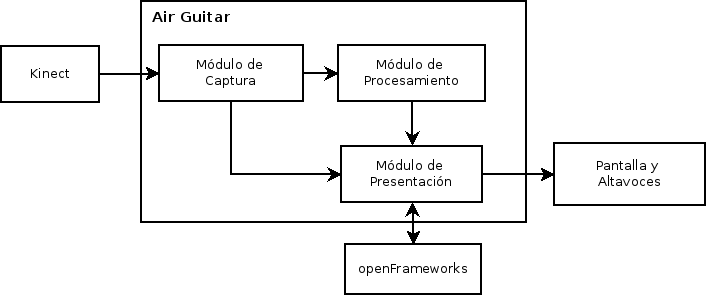
\includegraphics[width=0.8\textwidth]{../imagenes/diagrama_de_arquitectura.png}
        \caption{Diagrama de Arquitectura}
        \label{fig:arquitectura}
\end{figure}

\subsection{Enumeración de Módulos}
El cuadro~\ref{tab:modulos} muestra los módulos de la
figura~\ref{fig:arquitectura}. Por cada módulo se entrega un breve párrafo
descriptivo de su propósito, además de la sección en donde se especifica el
módulo en detalle.

\begin{table}[h]
        \centering
        \begin{tabular}{|p{3cm}|l|p{15mm}|}
                \hline
                \textbf{Módulo} & \textbf{Propósito} & \textbf{Sección} \\
                \hline
                Módulo de Captura & &\ref{sec:captura} \\
                \hline
                Módulo de Procesamiento & &\ref{sec:procesamiento}\\
                \hline
                Módulo de Presentación & &\ref{sec:presentacion}\\
                \hline
        \end{tabular}
        \caption{Módulos de la arquitectura del sistema}
        \label{tab:modulos}
\end{table}
\subsection{Matriz de Requisitos Funcionales y Módulos}

\section{Módulo de Captura}
\label{sec:captura}
\subsection{Definición de Módulo}
\begin{tabular}{p{2cm} l}
        \textbf{Propósito} & \\
        \textbf{Alcance} & \\
        \textbf{Dependencias} & \\
        \textbf{Supuestos} & \\
        \textbf{Restricciones} & \\
        \textbf{Estructura General} & \\
\end{tabular}
\subsection{Declaraciones Públicas}
Esta sección enumera constantes, tipos y variables del módulo, visibles para
otros módulos.
\subsubsection{Constantes Públicas}
\begin{tabular}{| p{30mm} | p{10cm} |}
        \hline
        \textbf{Nombre de la \mbox{constante}} & \textbf{Descripción} \\
        \hline
         & \\
        \hline
\end{tabular}
                

\subsubsection{Tipos de Datos Públicos}
\begin{tabular}{| p{30mm} | p{10cm} |}
        \hline
        \textbf{Nombre del \mbox{tipo}} & \textbf{Descripción} \\
        \hline
         & \\
        \hline
\end{tabular}
\subsubsection{Variables Públicos}
\begin{tabular}{| p{30mm} | p{10cm} |}
        \hline
        \textbf{Nombre de la \mbox{variable}} & \textbf{Descripción} \\
        \hline
         & \\
        \hline
\end{tabular}
\subsection{Funciones Públicas}
Las siguientes funciones son accesibles desde otros módulos. Otros módulos
tienen acceso a la funcionalidad de este módulo mediante estas funciones.
~\\

\begin{tabular}{| p{30mm} | p{10cm} |}
        \hline
        \textbf{Nombre de la \mbox{función}} & \textbf{Descripción breve} \\
        \hline
         & \\
        \hline
\end{tabular}
\subsection{Estructuras de Datos}
\subsection{Funciones Privadas}
Las siguientes funciones auxiliares son privadas de este módulo; otros módulos
no las pueden usar.
~\\

\begin{tabular}{| p{30mm} | p{10cm} |}
        \hline
        \textbf{Nombre de la \mbox{función}} & \textbf{Descripción breve} \\
        \hline
         & \\
        \hline
\end{tabular}
\subsection{Diseño Detallado de las Funciones}
\subsubsection{Función 1}
\begin{tabular}{p{2cm} l}
        \textbf{Propósito} & \\
        \textbf{Dependencias} & \\
        \textbf{Prototipo} & \\
        \textbf{Parámetro} & \textbf{Explicación} \\
        \begin{tabular}{p{2cm} l}
                Parámetro 1 & \\
        \end{tabular}

        \textbf{Retorno} & \\
        \textbf{Proceso} & Pseudocodigo \\
\end{tabular}


\section{Módulo de Procesamiento}
\label{sec:procesamiento}
\subsection{Definición de Módulo}
\begin{tabular}{p{2cm} l}
        \textbf{Propósito} & \\
        \textbf{Alcance} & \\
        \textbf{Dependencias} & \\
        \textbf{Supuestos} & \\
        \textbf{Restricciones} & \\
        \textbf{Estructura General} & \\
\end{tabular}
\subsection{Declaraciones Públicas}
Esta sección enumera constantes, tipos y variables del módulo, visibles para
otros módulos.
\subsubsection{Constantes Públicas}
\begin{tabular}{| p{30mm} | p{10cm} |}
        \hline
        \textbf{Nombre de la \mbox{constante}} & \textbf{Descripción} \\
        \hline
         & \\
        \hline
\end{tabular}
                

\subsubsection{Tipos de Datos Públicos}
\begin{tabular}{| p{30mm} | p{10cm} |}
        \hline
        \textbf{Nombre del \mbox{tipo}} & \textbf{Descripción} \\
        \hline
         & \\
        \hline
\end{tabular}
\subsubsection{Variables Públicos}
\begin{tabular}{| p{30mm} | p{10cm} |}
        \hline
        \textbf{Nombre de la \mbox{variable}} & \textbf{Descripción} \\
        \hline
         & \\
        \hline
\end{tabular}
\subsection{Funciones Públicas}
Las siguientes funciones son accesibles desde otros módulos. Otros módulos
tienen acceso a la funcionalidad de este módulo mediante estas funciones.
~\\

\begin{tabular}{| p{30mm} | p{10cm} |}
        \hline
        \textbf{Nombre de la \mbox{función}} & \textbf{Descripción breve} \\
        \hline
         & \\
        \hline
\end{tabular}
\subsection{Estructuras de Datos}
\subsection{Funciones Privadas}
Las siguientes funciones auxiliares son privadas de este módulo; otros módulos
no las pueden usar.
~\\

\begin{tabular}{| p{30mm} | p{10cm} |}
        \hline
        \textbf{Nombre de la \mbox{función}} & \textbf{Descripción breve} \\
        \hline
         & \\
        \hline
\end{tabular}
\subsection{Diseño Detallado de las Funciones}
\subsubsection{Función 1}
\begin{tabular}{p{2cm} l}
        \textbf{Propósito} & \\
        \textbf{Dependencias} & \\
        \textbf{Prototipo} & \\
        \textbf{Parámetro} & \textbf{Explicación} \\
        \begin{tabular}{p{2cm} l}
                Parámetro 1 & \\
        \end{tabular}

        \textbf{Retorno} & \\
        \textbf{Proceso} & Pseudocodigo \\
\end{tabular}


\section{Módulo de Presentación}
\label{sec:presentacion}
\subsection{Definición de Módulo}
\begin{tabular}{p{2cm} l}
        \textbf{Propósito} & \\
        \textbf{Alcance} & \\
        \textbf{Dependencias} & \\
        \textbf{Supuestos} & \\
        \textbf{Restricciones} & \\
        \textbf{Estructura General} & \\
\end{tabular}
\subsection{Declaraciones Públicas}
Esta sección enumera constantes, tipos y variables del módulo, visibles para
otros módulos.
\subsubsection{Constantes Públicas}
\begin{tabular}{| p{30mm} | p{10cm} |}
        \hline
        \textbf{Nombre de la \mbox{constante}} & \textbf{Descripción} \\
        \hline
         & \\
        \hline
\end{tabular}
                

\subsubsection{Tipos de Datos Públicos}
\begin{tabular}{| p{30mm} | p{10cm} |}
        \hline
        \textbf{Nombre del \mbox{tipo}} & \textbf{Descripción} \\
        \hline
         & \\
        \hline
\end{tabular}
\subsubsection{Variables Públicos}
\begin{tabular}{| p{30mm} | p{10cm} |}
        \hline
        \textbf{Nombre de la \mbox{variable}} & \textbf{Descripción} \\
        \hline
         & \\
        \hline
\end{tabular}
\subsection{Funciones Públicas}
Las siguientes funciones son accesibles desde otros módulos. Otros módulos
tienen acceso a la funcionalidad de este módulo mediante estas funciones.
~\\

\begin{tabular}{| p{30mm} | p{10cm} |}
        \hline
        \textbf{Nombre de la \mbox{función}} & \textbf{Descripción breve} \\
        \hline
         & \\
        \hline
\end{tabular}
\subsection{Estructuras de Datos}
\subsection{Funciones Privadas}
Las siguientes funciones auxiliares son privadas de este módulo; otros módulos
no las pueden usar.
~\\

\begin{tabular}{| p{30mm} | p{10cm} |}
        \hline
        \textbf{Nombre de la \mbox{función}} & \textbf{Descripción breve} \\
        \hline
         & \\
        \hline
\end{tabular}
\subsection{Diseño Detallado de las Funciones}
\subsubsection{Función 1}
\begin{tabular}{p{2cm} l}
        \textbf{Propósito} & \\
        \textbf{Dependencias} & \\
        \textbf{Prototipo} & \\
        \textbf{Parámetro} & \textbf{Explicación} \\
        \begin{tabular}{p{2cm} l}
                Parámetro 1 & \\
        \end{tabular}

        \textbf{Retorno} & \\
        \textbf{Proceso} & Pseudocodigo \\
\end{tabular}

\appendix 
\newpage

\addcontentsline{toc}{section}{Referencias}
\begin{thebibliography}{99}
% \bibitem{depth_range}\url{http://msdn.microsoft.com/en-us/library/hh973078.aspx#Depth_Ranges} \\
%         Microsoft Developer Network, 05 Nov 2013
% \bibitem{air_guitar}\url{https://en.wikipedia.org/wiki/Air_guitar#Contests} \\
%         Wikipedia, 05 Nov 2013
% \bibitem{kinect_spec}\url{http://msdn.microsoft.com/en-us/library/jj131033.aspx} \\
%         Microsoft Developer Network, 05 Nov 2013
% \bibitem{kinect_release}\url{http://en.wikipedia.org/wiki/Kinect#History} \\
%         Wikipedia, 05 Nov 2013
% \bibitem{sdk}\url{http://msdn.microsoft.com/en-us/library/hh855347.aspx} \\
%         Microsoft Developer Network, 05 Nov 2013
% \bibitem{kinect_new}\url{http://blogs.msdn.com/b/kinectforwindows/archive/2013/09/16/updated-sdk-with-html5-kinect-fusion-improvements-and-more.aspx} \\
%         Kinect for Windows Blog, 05 Noc 2013
\end{thebibliography}

\end{document} 
%%% Local Variables: %%% mode: latex %%% TeX-master: t %%% End:
